% !TeX spellcheck = it_IT
%Alberto Bobbo, Michele Bortone, Enrico Marcato
\documentclass[10pt, a4paper]{article}

\usepackage[scaled]{helvet}

\usepackage[utf8]{inputenc}
\usepackage[T1]{fontenc}
\usepackage[italian]{babel}

\usepackage{graphicx}
\usepackage{fix-cm}
\newcommand{\bigsize}{\fontsize{35pt}{20pt}\selectfont}
\newcommand{\mediumsize}{\fontsize{30pt}{20pt}\selectfont}
\newcommand{\normsize}{\fontsize{15pt}{10pt}\selectfont}


%crea uno spazio, utile perchè gli spazi extra dopo le macro
%vengono rimossi. Questo comando permette di inserirne uno.
\def\space{ }

\usepackage{float}
\usepackage{caption}

\usepackage{amsmath}
\usepackage{mathtools}

\usepackage{multirow}
%crea una cella per le tabelle in grado di andare a capo con \newline
%https://tex.stackexchange.com/questions/12703/how-to-create-fixed-width-table-columns-with-text-raggedright-centered-raggedlef
\usepackage{array}
\newcolumntype{L}[1]{>{\raggedright\let\newline\\\arraybackslash\hspace{0pt}}m{#1}}
\newcolumntype{C}[1]{>{\centering\let\newline\\\arraybackslash\hspace{0pt}}m{#1}}
\newcolumntype{R}[1]{>{\raggedleft\let\newline\\\arraybackslash\hspace{0pt}}m{#1}}

%puntini per l'indice
\usepackage{tocloft}
\renewcommand\cftsecleader{\cftdotfill{\cftdotsep}}


%https://tex.stackexchange.com/questions/4503/how-do-i-specify-color-in-rgb-using-hypersetup-in-hyperref
\usepackage{url}
\usepackage{breakurl}
\usepackage[colorlinks=true]{hyperref}
\usepackage[hyperref]{xcolor}
\definecolor{UniPD}{RGB}{155, 0, 20}
\definecolor{Crema}{RGB}{220, 197, 149}
\definecolor{LinkNormNoClick}{RGB}{0, 0, 238}
\definecolor{LinkNormClick}{RGB}{69, 123, 157}
\hypersetup{colorlinks,breaklinks,
	urlcolor=UniPD,
	linkcolor=UniPD}

%per alcune liste
\usepackage{blindtext}
\usepackage{scrextend}
\addtokomafont{labelinglabel}
{\sffamily}


\newcommand{\Componenti}{Alberto Bobbo \newline Michele Bortone \newline
	Enrico Marcato}
\newcommand{\Referente}{Alberto Bobbo \newline alberto.bobbo@studenti.math.unipd.it}
\newcommand{\Gruppo}{Bobbo, Bortone, Marcato}
\newcommand{\Titolo}{Relazione Progetto Tecnologie Web}

\usepackage{lastpage} %info sul # dell'ultima pagina del documento
\usepackage{fancyhdr} %per modificare dimensioni,margini, intestazioni e righe a piè di pagina
\fancypagestyle{plain}{
	% cancella tutti i campi di intestazione e piè di pagina
	\fancyhf{}
	
	\lfoot{ %piè di pagina
		\Titolo{} \ - \textit{\Gruppo{}}
	}
	\rfoot{Pagina \thepage{} di \pageref{LastPage}} %es: pag: 4 di 10
	
	%linea orizzontale alle posizioni top e bottom della pagina
	\renewcommand{\headrulewidth}{0pt}  
	\renewcommand{\footrulewidth}{0.3pt}
}
\pagestyle{plain}

\usepackage{listings}


\lstdefinelanguage{HTML5}{
	sensitive=true,
	keywords={
		%% JavaScript
		typeof, new, true, false, catch, function, return, null, catch, switch, var, if, in, while, do, else, case, break, foreach, as,
		%% HTML
		html, meta, style, head, body, script, canvas, h1, h2, h3, h4, h5, h6, table, thead, tbody, tfoot, p, a, div, input, form, tr, th, label, ?php, ?, 
		%% CSS
		border:, transform:, -moz-transform:, transition-duration:, transition-property:,
		transition-timing-function:
	},
	% http://texblog.org/tag/otherkeywords/
	keywords=[2]{<, >, \, /, />, </ },  %%tag
	keywords=[3]{href, title, label, aria-label, lang, for, tabindex, placeholder, id, type, value, class, scope, }, %%attributi
	ndkeywords={class, export, boolean, throw, implements, import, this},
	keywords=[4]{echo, print\_ordinable\_th, REQUIRED},
	comment=[l]{//},
	% morecomment=[s][keywordstyle]{<}{>},  
	morecomment=[s]{/*}{*/},
	morecomment=[s]{<!}{>},
	morestring=[b]',
	morestring=[b]",    
	alsoletter={-},
	alsodigit={:}
}

\lstset{
	backgroundcolor=\color{background},
	tabsize=4,    
	language=HTML5,
	basicstyle=\ttfamily\linespread{1.15}\footnotesize,
	upquote=true,
	aboveskip={1.5},
	columns=fixed,
	showstringspaces=false,
	extendedchars=true,
	inputencoding=utf8,
	breaklines=true,
	prebreak = \raisebox{0ex}[0ex][0ex]{\ensuremath{\hookleftarrow}},
	frame=none,
	numbers=left,
	numbersep=5pt,	
	showtabs=false,
	showspaces=false,
	showstringspaces=false,
	basicstyle=\tiny\color{normal},
	identifierstyle=\color{normal},
	keywordstyle=\color{purple},
	keywordstyle=[2]\color{normal},
	keywordstyle=[3]\color{identifier},
	keywordstyle=[4]\color{blue},
	commentstyle=\color{comment},
	stringstyle=\color{string},
	numberstyle=\tiny\color{background}.
}



\begin{document}


\begin{titlepage}
\centering


\includegraphics[width=50mm]{Images/logo.png}
\vspace*{30px}
{\Large \\ \textbf{RELAZIONE PROGETTO TECNOLOGIE WEB}\\}
\vspace*{30px}

\bgroup
\def\arraystretch{1.3}
\centering

\begin{tabular}{c|L{5cm}}
\multicolumn{2}{c}{} \\ 
  \textbf{Componenti} & \Componenti{} \\
  \textbf{Referente} & \Referente{}
\end{tabular}
\egroup



\vspace*{80px}


\hypersetup{hidelinks}
\bgroup
\def\arraystretch{1.3}
\centering
\begin{tabular}{c}
\multicolumn{1}{c}{\textbf{Indirizzo Web Del Sito} } \\
  \url{http://tecweb2016.studenti.math.unipd.it/abobbo/pages/home.php}
\end{tabular}
\egroup

\vspace*{80px}

\begin{tabular}{c|L{4cm}}
\multicolumn{2}{c}{\textbf{Credenziali Admin} } \\ \hline
  \textbf{Username} & admin@progetto.com \\
  \textbf{Password} & admin
\end{tabular}
\quad
\begin{tabular}{c|L{4cm}}
\multicolumn{2}{c}{\textbf{Credenziali Utente} } \\ \hline
 \textbf{Username} & gino@progetto.com \\
  \textbf{Password} & ciaog
\end{tabular}

\vspace*{10px}

\end{titlepage}


\newpage
\hypersetup{hidelinks}
\tableofcontents
\newpage
\section{Presentazione sito}
Il sito in questione ha lo scopo di presentare l'evento musicale "Home Festival". Qui l'utente può trovare tutte le informazioni di cui ha bisogno per assistere ai vari concerti che avranno luogo durante il festival: in particolare vengono descritti brevemente i gruppi che parteciperanno all'evento ed è inoltre presente un insieme di indicazioni per raggiungere il luogo dell'evento con i principali mezzi di trasporto.
È anche possibile effettuare una registrazione, che permette all'utente di commentare le ultime news, sugli artisti partecipanti al festival, pubblicate dagli amministratori. 
\section{Utenti destinatari}
Il sito è destinato a tutti gli utenti che intendono partecipare all’Home Festival o che comunque desiderano avere informazioni riguardo all’evento.  
All’interno del footer sono inoltre presenti alcuni contatti, nel caso l’utente volesse ricevere informazioni aggiuntive, e i link alle pagine dei principali social network, dove vengono inseriti gli ultimi aggiornamenti riguardanti il festival.
\section{Tipi di utenti}
Le categorie di utenti che il sito mette a disposizione sono:
\newline \textbf{Amministratore: }è in grado di pubblicare gli articoli che verranno inseriti nella sezione News tramite una form presente nella pagina stessa. Può inoltre rimuovere i commenti pubblicati dagli utenti sui vari articoli presenti sul sito e commentare a sua volta.
\newline \textbf{Utente: }rappresenta l'utilizzatore vero e proprio del sito. Può commentare gli articoli pubblicati nelle News dagli amministratori.
\section{Progettazione}
\subsection{Organizzazione del sito}
Il sito presenta una barra di navigazione globale che contiene le varie aree del sito (Home, News, LineUp, Biglietti, Come Arrivare, Orari, Login e Registrati) e una barra di ricerca, utile per l'individuazione di particolari informazioni all'interno dell'intero sito.
Il codice della barra di navigazione è contenuto nel file nav.php, che viene richiamato da tutte le pagine del sito.
%%\begin{figure}[h!]
%%  \centering
%%  
\includegraphics[width=1\textwidth]{Images/navbar.png}
%%  \caption{Barra di navigazione globale e barra di ricerca}
%%  \label{fig:navbar}
%%\end{figure}
\subsection{Aree del sito}
\textbf{Home: }è la homepage del sito. La pagina è generata dinamicamente dal file home.php e presenta una form che permette agli utenti di iscriversi alla newsletter, una sezione dove viene visualizzato l'ultimo articolo inserito dagli amministratori e un'immagine che elenca i vari artisti che partecipano al festival musicale.
\newline \textbf{News: }contiene tutti gli articoli pubblicati sul sito. In ogni pagina sono visualizzati 5 articoli ed è possibile navigare tra le varie pagine tramite il menu di paginazione posizionato in coda alle news. L'utente può inoltre cliccare su singolo articolo per visualizzarne la versione completa e, se ha anche effettuato il login al sito, può scrivere un commento tramite il form apposito. La pagina viene generata dinamicamente dal file news.php, in modo da mantenere l'ordine cronologico degli articoli visualizzati.
%%\begin{figure}[h!]
%%  \centering
%%  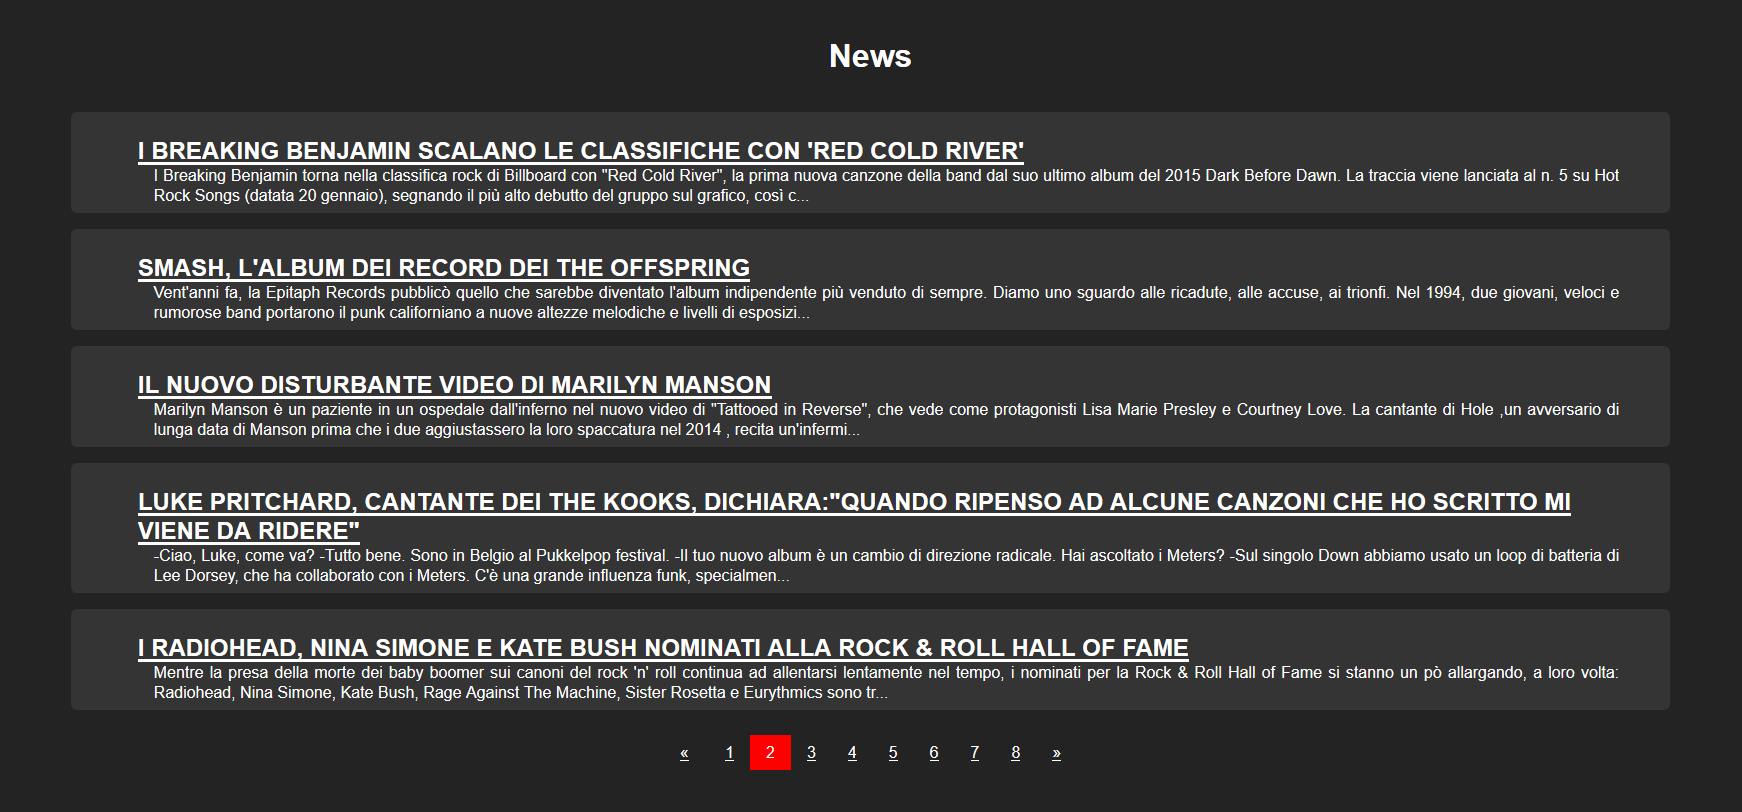
\includegraphics[width=1\textwidth]{Images/news.png}
%%  \caption{Pagina per la visualizzazione delle news}
%%  \label{fig:news}
%%\end{figure}
%%\begin{figure}[h!]
%%  \centering
%%  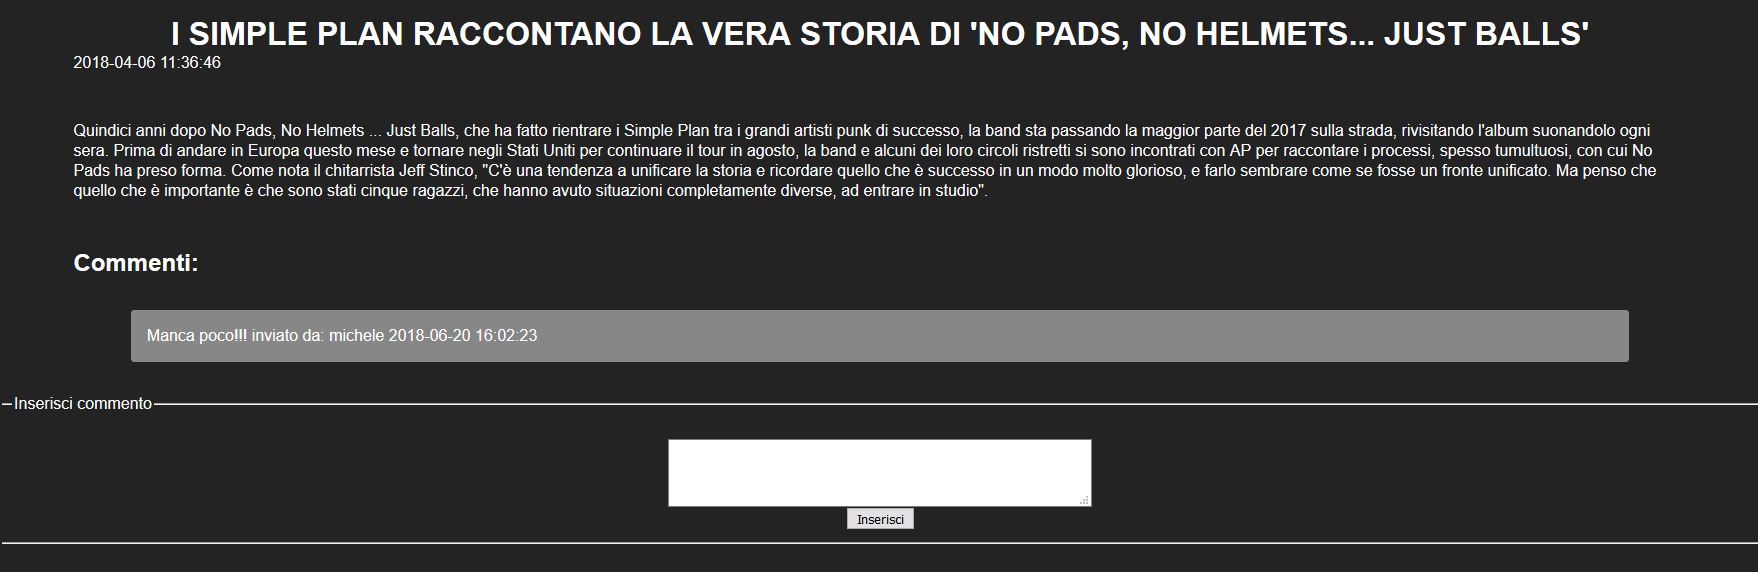
\includegraphics[width=1\textwidth]{Images/articolo.png}
%%  \caption{Pagina per la visualizzazione di un articolo con relativo form per l'inserimento di commenti}
%%  \label{fig:articolo}
%%\end{figure}
\newline \textbf{LineUp: }presenta l'insieme degli artisti che partecipano all'evento, descritti da relativi immagini e nomi. Cliccando su quest'ultimo è possibile accedere alla pagina dedicata al singolo artista, che contiene una breve descrizione della sua carriera e alcune informazioni generali.
%%\begin{figure}[h!]
%%  \centering
%%  \includegraphics[width=1\textwidth]{Images/lineup.png}
%%  \caption{}
%%  \label{fig:lineup}
%%\end{figure}
%%\begin{figure}[h!]
%%  \centering
%%  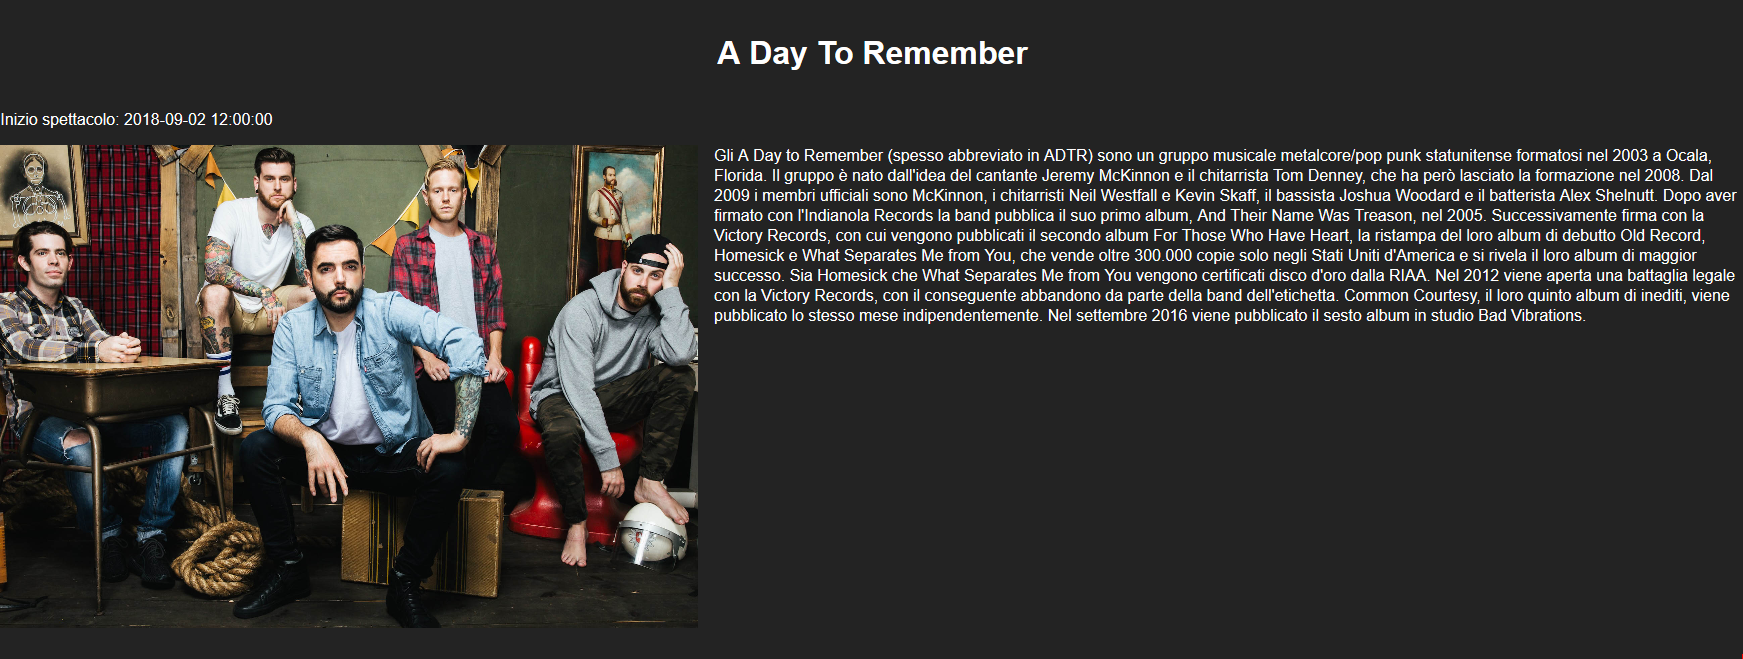
\includegraphics[width=1\textwidth]{Images/artista.png}
%%  \caption{}
%%  \label{fig:artista}
%%\end{figure}
\newline \textbf{Biglietti: }fornisce all'utente le tipologie di biglietto che è possibile acquistare con una breve descrizione sottostante e il relativo prezzo.
%%\begin{figure}[h!]
%%  \centering
%%  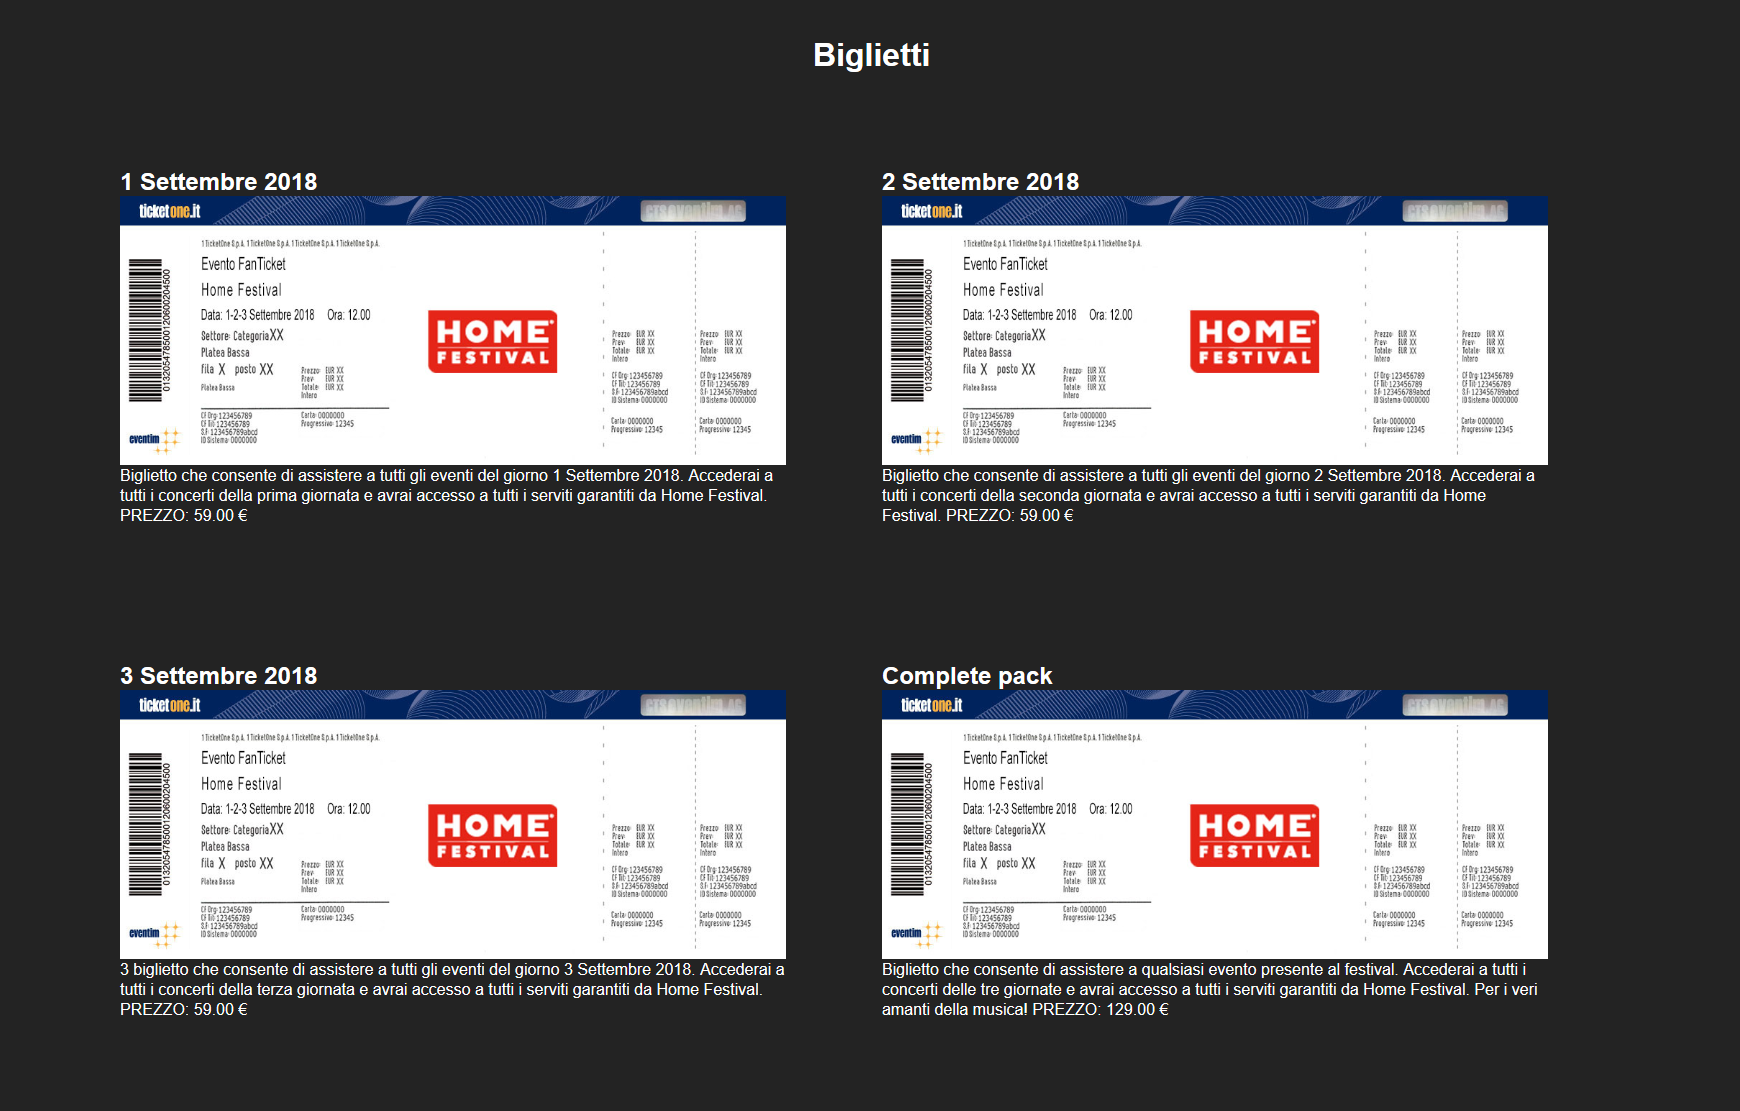
\includegraphics[width=1\textwidth]{Images/biglietti.png}
%%  \caption{Pagina con i vari tipi di biglietto proposti per poter partecipare al festival}
%%  \label{fig:biglietti}
%%\end{figure}
\newline \textbf{Come Arrivare: }contiene una descrizione testuale delle indicazioni per raggiungere il luogo dell'evento con i principali mezzi di trasporto. Non è stata inserita una mappa per mantenere le informazioni della pagina il più accessibili possibili.
%%\begin{figure}[h!]
%%  \centering
%% 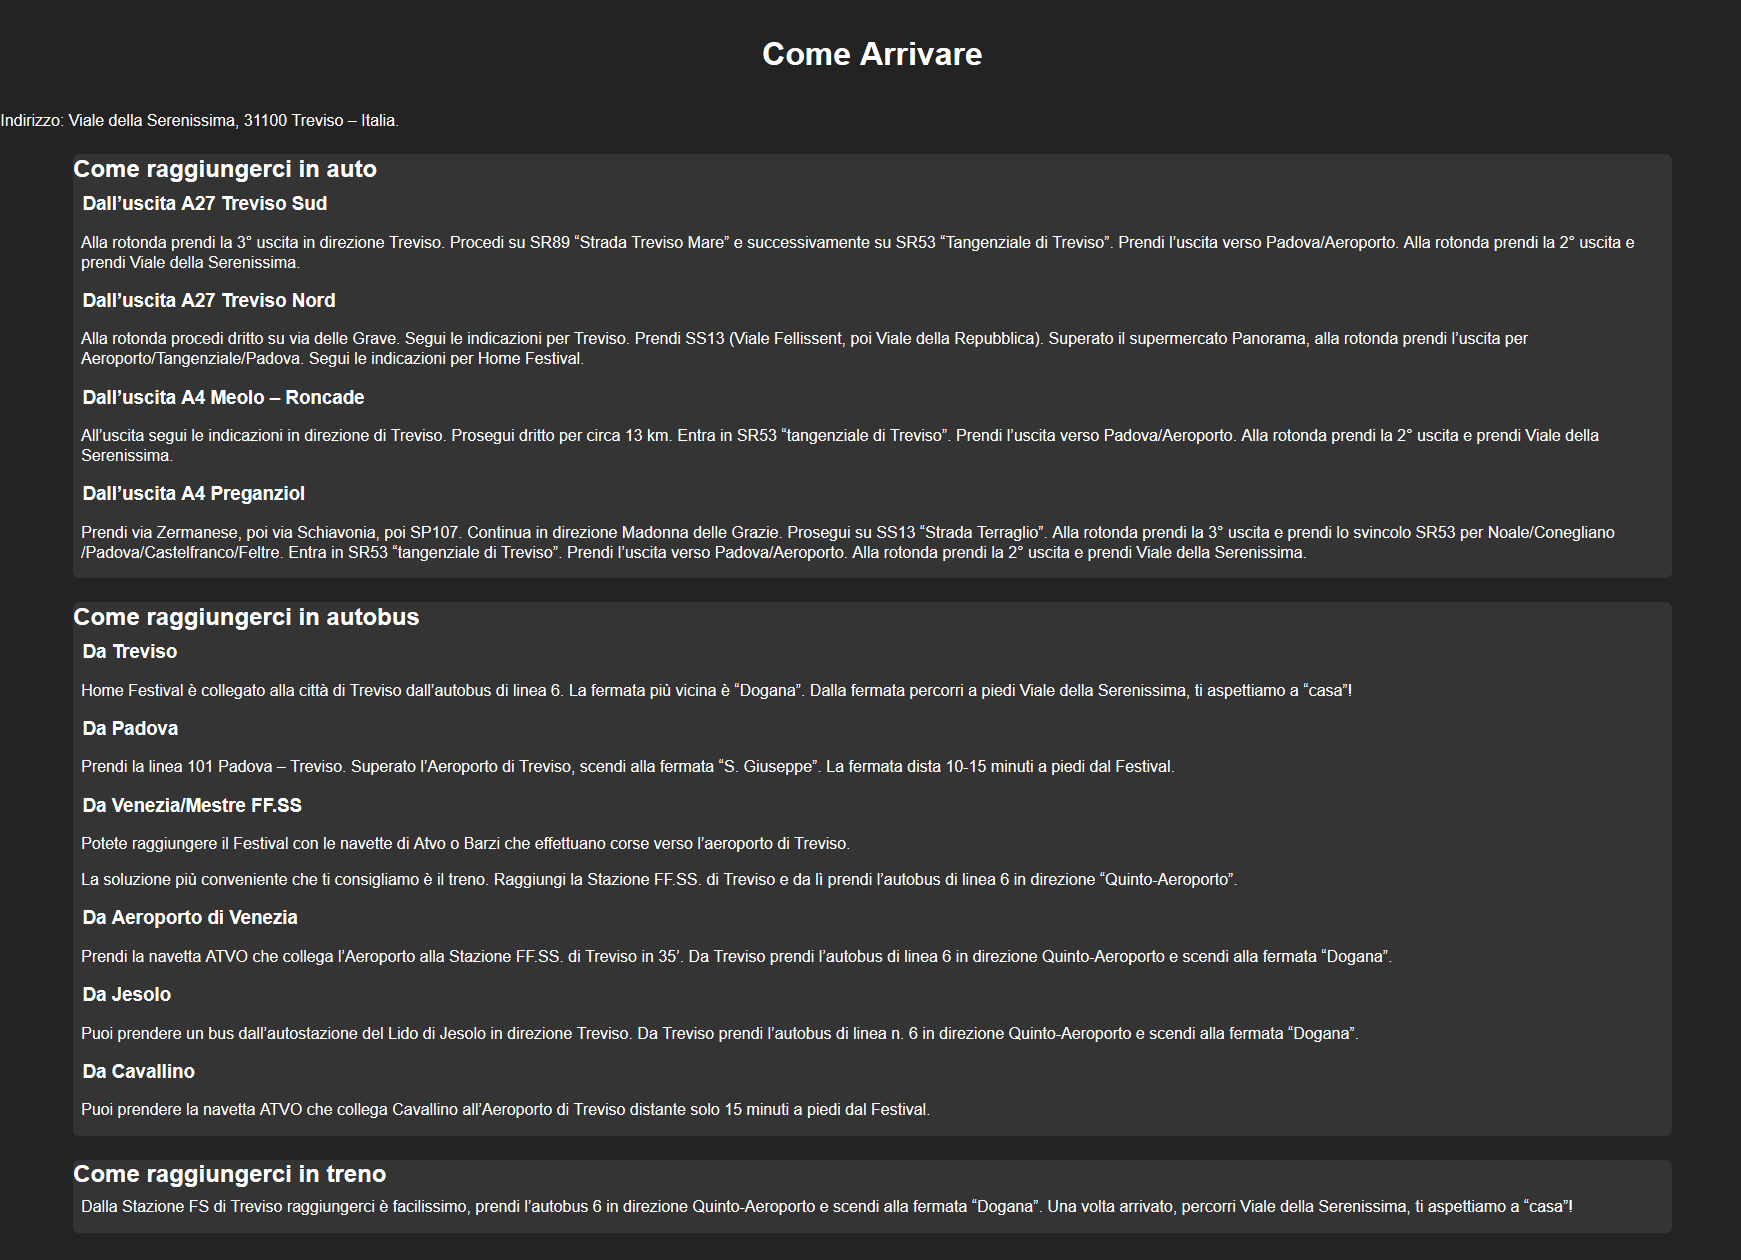
\includegraphics[width=1\textwidth]{Images/indicazioni.png}
%%  \caption{Indicazioni per raggiungere il festival}
%%  \label{fig:indicazioni}
%%\end{figure}
\newline \textbf{Orari: }presenta gli orari dei vari concerti che avranno luogo durante il festival suddivisi per giornate.
%%\begin{figure}[h!]
%% \centering
%%  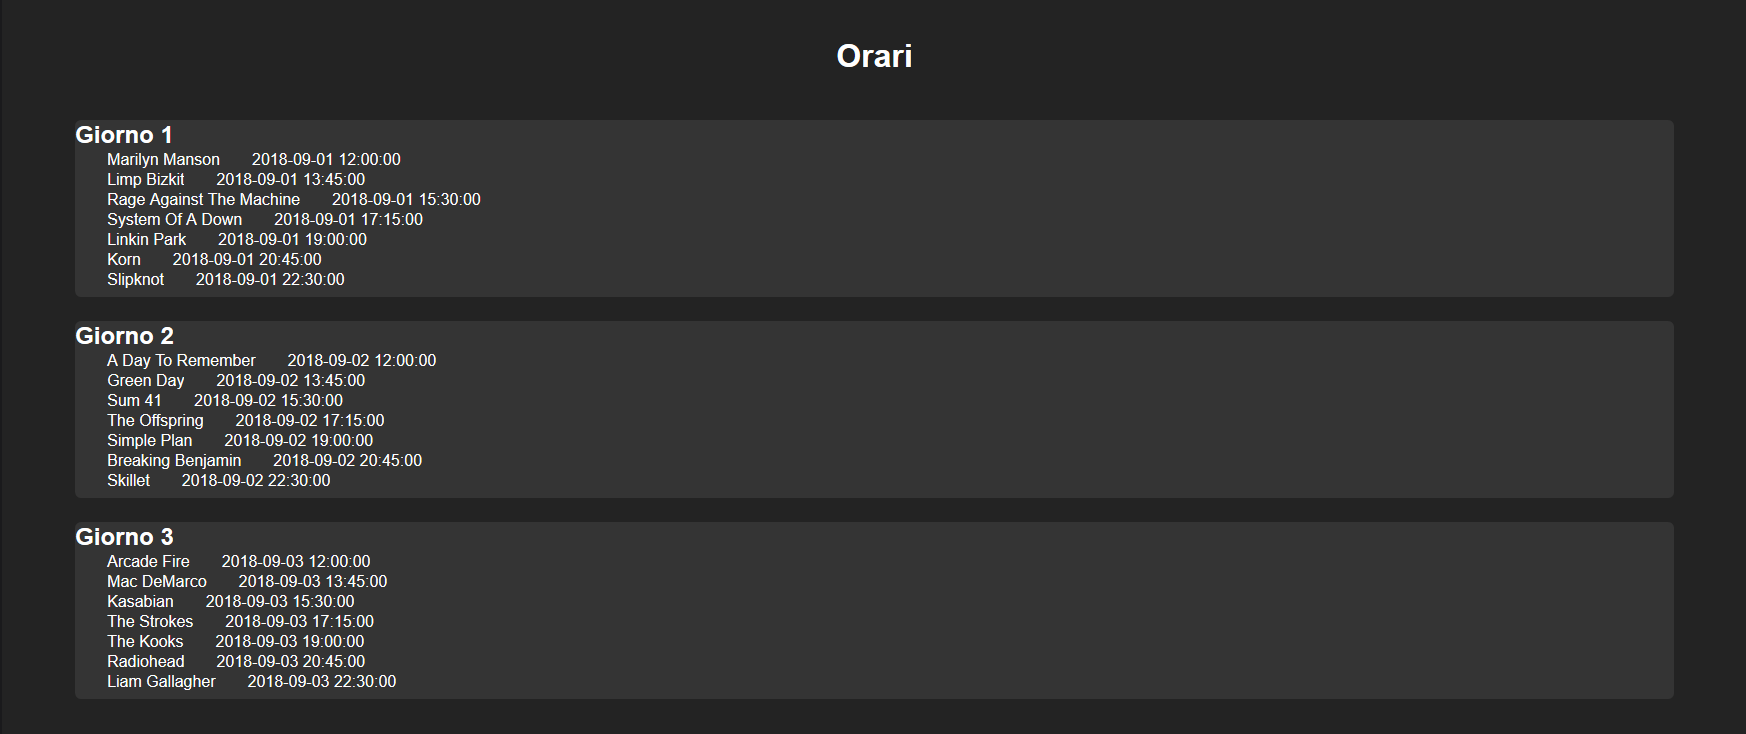
\includegraphics[width=1\textwidth]{Images/orari.png}
%%  \caption{Orari dei concerti che si tengono nelle 3 giornate del festival}
%%  \label{fig:orari}
%%\end{figure}
%%\pagebreak
\newline \textbf{Login: }fornisce una form, sia agli utenti che agli amministratori, per effettuare il login al sito. Dopo aver completato l'accesso, l'utente può commentare gli articoli del sito mentre gli amministratori possono anche eliminare i commenti e gli articoli inseriti.
%%\begin{figure}[h!]
%% \centering
%%  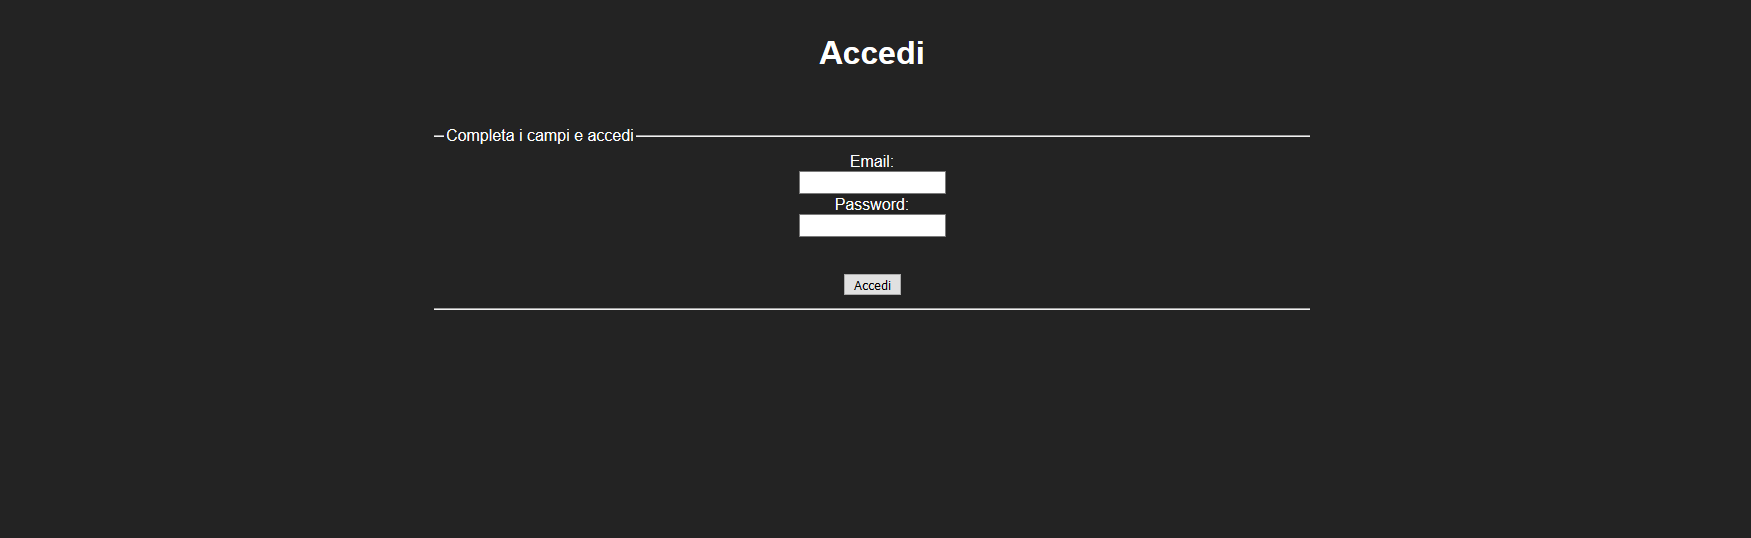
\includegraphics[width=1\textwidth]{Images/login.png}
%%  \caption{}
%%  \label{fig:login}
%%\end{figure}
\newline \textbf{Registrati: }contiene una form che consente all'utente di effettuare la registrazione al sito inserendo i propri dati. Dopo che si è registrato, l'utente può accedere al sito con l'account che ha appena creato.
%%\begin{figure}[h!]
%% \centering
%%  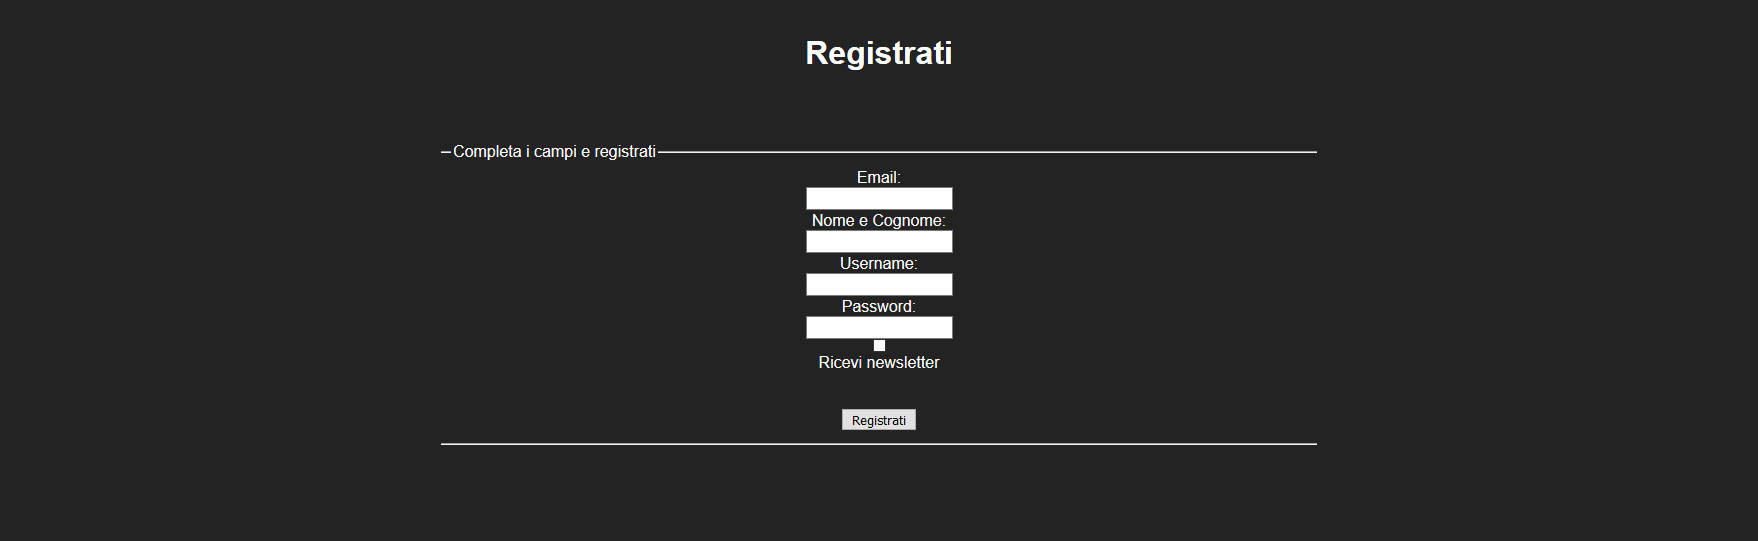
\includegraphics[width=1\textwidth]{Images/registrazione.png}
%%  \caption{}
%%  \label{fig:registrazione}
%%\end{figure}
\subsection{Struttura organizzativa}
Come struttura organizzativa è stato impiegato un database, dato che ogni elemento presente sul sito (utenti, articoli, commenti, artisti e biglietti), può essere ricondotto a un'entità all'interno della base di dati. Questo facilità la gestione e l'inserimento dei dati all'interno del sito.
\section{Accessibilità}

\subsection{Perceivable}


\subsubsection{Text Alternatives}
Tutti i contenuti non testuali presenti sul sito dispongono di un'alternativa testuale: le varie immagini inserite presentano tutte l'attributo \textbf{alt}, mentre la mappa che viene visualizzata nella pagina Come Arrivare possiede una descrizione testuale sottostante, nel caso venisse utilizzato uno screen reader per visitare il sito oppure JavaScript fosse disattivato.

\subsubsection{Time-based Media}
I contenuti temporali all'interno di un sito risultano poco accessibili agli utenti con disabilità e per questo non sono stati inseriti.

\subsubsection{Adaptability}
Il sito può essere visualizzato su diversi dispositivi con dimensioni dello schermo differenti mantenendo sempre una struttura simile e non perdendo alcuna informazione. La versione per smartphone si differenzia dalle versioni desktop e tablet soprattutto per la navbar, la quale mantiene il logo del festival e la barra di ricerca, che hanno un'importanza prioritaria, mentre il menu per navigare all'interno sito viene sostituito da un unico bottone che, quando viene effettuato un tap, rende visibili le varie voci del menu. Per motivi di impaginazione, inoltre, negli smartphone non è presente l’immagine di testata.

\subsection{Understandable}

\subsubsection{Legibility}
Il testo inserito nel sito rimane sempre leggibile in quanto è stato utilizzato un colore per lo sfondo che ha un contrasto elevato con tutti gli elementi testuali presenti nelle varie pagine. Il sito è inoltre scritto con codifica UTF-8.


\subsubsection{Predictability}


\subsubsection{Input Assistance}
Al momento della registrazione, dell’accesso al sito tramite credenziali e dell’iscrizione alla newsletter, i campi inseriti devono rispettare delle parametri per essere accettati dal server. L’utente, mentre esegue queste azioni, visualizza dei messaggi al di sotto dei textfield che lo aiutano attraverso la procedura.

\subsection{Robust}

\subsubsection{Compatibility}
Il sito è stato sviluppato utilizzando XHTML 1.0 e CSS 3.0

\subsection{Operable}

\subsubsection{Keyboard Accessibility}
È possibile navigare sul sito e compilare i vari form proposti utilizzando il tasto \textbf{TAB}. Le voci della navbar dispongono inoltre di access key, le quali facilitano la navigazione tramite screen reader.

\subsubsection{Time Availability}
Nel sito non sono stati inseriti contenuti temporizzati in quanto questi non risulterebbero usufruibili da tutti i visitatori del sito.

\subsubsection{Epilepsy}
Il sito non presenta contenuti che potrebbero creare problemi agli utenti affetti da epilessia.

\subsubsection{Navigability}
All'inizio di ogni pagina è stato inserito un link che rimanda direttamente al contenuto della stessa, trascurando la navbar e la barra di ricerca, in modo da facilitare la navigazione agli utenti non vedenti che utilizzano uno screen reader.

\subsection{Visione del sito da parte di individui con disturbi visivi}

\subsubsection{Deuteranopia}

\subsubsection{Protanopia}

\subsubsection{Tritanopia}

\subsection{Sintetizzatore vocale}

\section{Usabilità}

\subsection{Link}

\subsection{Navbar}

\section{Amministratore, utente}

\subsection{Amministratore}

\subsection{Utente}

\section{Scelte Progettuali}
\begin{itemize}
	\item{Il form per l'inserimento di un articolo da parte dell'amministratore, che viene visualizzato se quest'ultimo ha effettuato il login, è posto al termine della pagina News, e non all'inizio, per favorire il controllo dell'articolo che è appena stato inserito}
	\item{Posizione form commento articolo...........................}
	\item{Link pagination non risultano visitati.....................................}
\end{itemize}

\section{Gerarchia dei file}
I file che compongono il sito sono contenuti nella cartella \textbf{public\textunderscore html} mentre le sessioni PHP sono salvate nella cartella \textbf{php\textunderscore sessions}. All'interno della cartella \textbf{public\textunderscore html} sono presenti il file index.html, utilizzato per effettuare il redirect a home.php, e alcune sotto cartelle indicate di seguito:
\begin{itemize}
  \item{\textbf{css}: contiene i file css utili alla presentazione del sito}
    \begin{itemize}
      \item{print.css: file css per la presentazione del sito su tutti i dispositivi}
      \item{style.css: file css per la stampa delle pagine}
    \end{itemize}
  \item{\textbf{images}: contiene}
    \begin{itemize}
       \item{Le immagini utilizzate nelle varie pagine del sito}
        \item{La cartella GroupsPic, dove sono presenti le immagini utilizzate nelle pagina LineUp}
    \end{itemize}
  \item{\textbf{js}: contiene il file javascript Script.js}
  \item{\textbf{layout}: contiene i file }
    \begin{itemize}
       \item{footer.php: file utilizzato da tutte le pagine per modellare il footer}
        \item{header.html: file utilizzato da tutte le pagine per modellare l'header}
        \item{nav.html: file utilizzato da tutte le pagine per modellare la barra di navigazione}
    \end{itemize}
  \item{\textbf{pages}: contiene i file PHP che compongono le pagine del sito}
\end{itemize}
\section{XHTML}

\section{PHP}

\section{Javascript}

\section{Validazione}

\section{Compatibilità browser}

\subsection{Compatibilità con Internet Explorer}

\subsubsection{Internet Explorer 8}

\subsubsection{Internet Explorer 11}

\subsection{Compatibilità con Microsoft Edge}

\subsection{Compatibilità con Opera}

\subsection{Compatibilità con Safari}

\subsection{Compatibilità con Chrome}

\subsection{Compatibilità con Firefox}

\subsection{Dispositivi Mobili}

asdasdasd
\section{Organizzazione}

\begin{labeling}{alligator}
	\item[\textbf{Alberto Bobbo}] \item[] %serve perché altrimenti il primo elemento della lista inizia su questa linea
		\begin{itemize}
			\item{Creazione e reperimento dei contenuti multimediali}
			\item{Codice HTML }
			\item{Codice CSS per la presentazione}
			\item{Validazione codice e correzione errori}
		\end{itemize}
	\item[\textbf{Michele Bortone}] \item[]
		\begin{itemize}
			\item{Codice HTML}
			\item{Creazione e gestione del database}
			\item{Codice PHP per la gestione dinamica dei contenuti}
			\item{Test funzionalità del sito su vari dispositivi e browser}
		\end{itemize}
	\item[\textbf{Enrico Marcato}] \item[]
		\begin{itemize}
			\item{Codice HTML }
			\item{Codice CSS per la presentazione}
			\item{Codice CSS per la stampa}
			\item{Codice PHP per la sessione utente   }
		\end{itemize}
\end{labeling}







































\end{document}